% Options for packages loaded elsewhere
\PassOptionsToPackage{unicode}{hyperref}
\PassOptionsToPackage{hyphens}{url}
\PassOptionsToPackage{dvipsnames,svgnames,x11names}{xcolor}
%
\documentclass[
  letterpaper,
  DIV=11,
  numbers=noendperiod]{scrartcl}

\usepackage{amsmath,amssymb}
\usepackage{iftex}
\ifPDFTeX
  \usepackage[T1]{fontenc}
  \usepackage[utf8]{inputenc}
  \usepackage{textcomp} % provide euro and other symbols
\else % if luatex or xetex
  \usepackage{unicode-math}
  \defaultfontfeatures{Scale=MatchLowercase}
  \defaultfontfeatures[\rmfamily]{Ligatures=TeX,Scale=1}
\fi
\usepackage{lmodern}
\ifPDFTeX\else  
    % xetex/luatex font selection
\fi
% Use upquote if available, for straight quotes in verbatim environments
\IfFileExists{upquote.sty}{\usepackage{upquote}}{}
\IfFileExists{microtype.sty}{% use microtype if available
  \usepackage[]{microtype}
  \UseMicrotypeSet[protrusion]{basicmath} % disable protrusion for tt fonts
}{}
\makeatletter
\@ifundefined{KOMAClassName}{% if non-KOMA class
  \IfFileExists{parskip.sty}{%
    \usepackage{parskip}
  }{% else
    \setlength{\parindent}{0pt}
    \setlength{\parskip}{6pt plus 2pt minus 1pt}}
}{% if KOMA class
  \KOMAoptions{parskip=half}}
\makeatother
\usepackage{xcolor}
\usepackage{svg}
\setlength{\emergencystretch}{3em} % prevent overfull lines
\setcounter{secnumdepth}{-\maxdimen} % remove section numbering
% Make \paragraph and \subparagraph free-standing
\makeatletter
\ifx\paragraph\undefined\else
  \let\oldparagraph\paragraph
  \renewcommand{\paragraph}{
    \@ifstar
      \xxxParagraphStar
      \xxxParagraphNoStar
  }
  \newcommand{\xxxParagraphStar}[1]{\oldparagraph*{#1}\mbox{}}
  \newcommand{\xxxParagraphNoStar}[1]{\oldparagraph{#1}\mbox{}}
\fi
\ifx\subparagraph\undefined\else
  \let\oldsubparagraph\subparagraph
  \renewcommand{\subparagraph}{
    \@ifstar
      \xxxSubParagraphStar
      \xxxSubParagraphNoStar
  }
  \newcommand{\xxxSubParagraphStar}[1]{\oldsubparagraph*{#1}\mbox{}}
  \newcommand{\xxxSubParagraphNoStar}[1]{\oldsubparagraph{#1}\mbox{}}
\fi
\makeatother

\usepackage{color}
\usepackage{fancyvrb}
\newcommand{\VerbBar}{|}
\newcommand{\VERB}{\Verb[commandchars=\\\{\}]}
\DefineVerbatimEnvironment{Highlighting}{Verbatim}{commandchars=\\\{\}}
% Add ',fontsize=\small' for more characters per line
\usepackage{framed}
\definecolor{shadecolor}{RGB}{241,243,245}
\newenvironment{Shaded}{\begin{snugshade}}{\end{snugshade}}
\newcommand{\AlertTok}[1]{\textcolor[rgb]{0.68,0.00,0.00}{#1}}
\newcommand{\AnnotationTok}[1]{\textcolor[rgb]{0.37,0.37,0.37}{#1}}
\newcommand{\AttributeTok}[1]{\textcolor[rgb]{0.40,0.45,0.13}{#1}}
\newcommand{\BaseNTok}[1]{\textcolor[rgb]{0.68,0.00,0.00}{#1}}
\newcommand{\BuiltInTok}[1]{\textcolor[rgb]{0.00,0.23,0.31}{#1}}
\newcommand{\CharTok}[1]{\textcolor[rgb]{0.13,0.47,0.30}{#1}}
\newcommand{\CommentTok}[1]{\textcolor[rgb]{0.37,0.37,0.37}{#1}}
\newcommand{\CommentVarTok}[1]{\textcolor[rgb]{0.37,0.37,0.37}{\textit{#1}}}
\newcommand{\ConstantTok}[1]{\textcolor[rgb]{0.56,0.35,0.01}{#1}}
\newcommand{\ControlFlowTok}[1]{\textcolor[rgb]{0.00,0.23,0.31}{\textbf{#1}}}
\newcommand{\DataTypeTok}[1]{\textcolor[rgb]{0.68,0.00,0.00}{#1}}
\newcommand{\DecValTok}[1]{\textcolor[rgb]{0.68,0.00,0.00}{#1}}
\newcommand{\DocumentationTok}[1]{\textcolor[rgb]{0.37,0.37,0.37}{\textit{#1}}}
\newcommand{\ErrorTok}[1]{\textcolor[rgb]{0.68,0.00,0.00}{#1}}
\newcommand{\ExtensionTok}[1]{\textcolor[rgb]{0.00,0.23,0.31}{#1}}
\newcommand{\FloatTok}[1]{\textcolor[rgb]{0.68,0.00,0.00}{#1}}
\newcommand{\FunctionTok}[1]{\textcolor[rgb]{0.28,0.35,0.67}{#1}}
\newcommand{\ImportTok}[1]{\textcolor[rgb]{0.00,0.46,0.62}{#1}}
\newcommand{\InformationTok}[1]{\textcolor[rgb]{0.37,0.37,0.37}{#1}}
\newcommand{\KeywordTok}[1]{\textcolor[rgb]{0.00,0.23,0.31}{\textbf{#1}}}
\newcommand{\NormalTok}[1]{\textcolor[rgb]{0.00,0.23,0.31}{#1}}
\newcommand{\OperatorTok}[1]{\textcolor[rgb]{0.37,0.37,0.37}{#1}}
\newcommand{\OtherTok}[1]{\textcolor[rgb]{0.00,0.23,0.31}{#1}}
\newcommand{\PreprocessorTok}[1]{\textcolor[rgb]{0.68,0.00,0.00}{#1}}
\newcommand{\RegionMarkerTok}[1]{\textcolor[rgb]{0.00,0.23,0.31}{#1}}
\newcommand{\SpecialCharTok}[1]{\textcolor[rgb]{0.37,0.37,0.37}{#1}}
\newcommand{\SpecialStringTok}[1]{\textcolor[rgb]{0.13,0.47,0.30}{#1}}
\newcommand{\StringTok}[1]{\textcolor[rgb]{0.13,0.47,0.30}{#1}}
\newcommand{\VariableTok}[1]{\textcolor[rgb]{0.07,0.07,0.07}{#1}}
\newcommand{\VerbatimStringTok}[1]{\textcolor[rgb]{0.13,0.47,0.30}{#1}}
\newcommand{\WarningTok}[1]{\textcolor[rgb]{0.37,0.37,0.37}{\textit{#1}}}

\providecommand{\tightlist}{%
  \setlength{\itemsep}{0pt}\setlength{\parskip}{0pt}}\usepackage{longtable,booktabs,array}
\usepackage{calc} % for calculating minipage widths
% Correct order of tables after \paragraph or \subparagraph
\usepackage{etoolbox}
\makeatletter
\patchcmd\longtable{\par}{\if@noskipsec\mbox{}\fi\par}{}{}
\makeatother
% Allow footnotes in longtable head/foot
\IfFileExists{footnotehyper.sty}{\usepackage{footnotehyper}}{\usepackage{footnote}}
\makesavenoteenv{longtable}
\usepackage{graphicx}
\makeatletter
\newsavebox\pandoc@box
\newcommand*\pandocbounded[1]{% scales image to fit in text height/width
  \sbox\pandoc@box{#1}%
  \Gscale@div\@tempa{\textheight}{\dimexpr\ht\pandoc@box+\dp\pandoc@box\relax}%
  \Gscale@div\@tempb{\linewidth}{\wd\pandoc@box}%
  \ifdim\@tempb\p@<\@tempa\p@\let\@tempa\@tempb\fi% select the smaller of both
  \ifdim\@tempa\p@<\p@\scalebox{\@tempa}{\usebox\pandoc@box}%
  \else\usebox{\pandoc@box}%
  \fi%
}
% Set default figure placement to htbp
\def\fps@figure{htbp}
\makeatother

\KOMAoption{captions}{tableheading}
\makeatletter
\@ifpackageloaded{caption}{}{\usepackage{caption}}
\AtBeginDocument{%
\ifdefined\contentsname
  \renewcommand*\contentsname{Índice}
\else
  \newcommand\contentsname{Índice}
\fi
\ifdefined\listfigurename
  \renewcommand*\listfigurename{Lista de Figuras}
\else
  \newcommand\listfigurename{Lista de Figuras}
\fi
\ifdefined\listtablename
  \renewcommand*\listtablename{Lista de Tabelas}
\else
  \newcommand\listtablename{Lista de Tabelas}
\fi
\ifdefined\figurename
  \renewcommand*\figurename{Figura}
\else
  \newcommand\figurename{Figura}
\fi
\ifdefined\tablename
  \renewcommand*\tablename{Tabela}
\else
  \newcommand\tablename{Tabela}
\fi
}
\@ifpackageloaded{float}{}{\usepackage{float}}
\floatstyle{ruled}
\@ifundefined{c@chapter}{\newfloat{codelisting}{h}{lop}}{\newfloat{codelisting}{h}{lop}[chapter]}
\floatname{codelisting}{Listagem}
\newcommand*\listoflistings{\listof{codelisting}{Lista de Listagens}}
\makeatother
\makeatletter
\makeatother
\makeatletter
\@ifpackageloaded{caption}{}{\usepackage{caption}}
\@ifpackageloaded{subcaption}{}{\usepackage{subcaption}}
\makeatother

\ifLuaTeX
\usepackage[bidi=basic]{babel}
\else
\usepackage[bidi=default]{babel}
\fi
\babelprovide[main,import]{portuguese}
% get rid of language-specific shorthands (see #6817):
\let\LanguageShortHands\languageshorthands
\def\languageshorthands#1{}
\usepackage{bookmark}

\IfFileExists{xurl.sty}{\usepackage{xurl}}{} % add URL line breaks if available
\urlstyle{same} % disable monospaced font for URLs
\hypersetup{
  pdftitle={Aula 2 - Parte 2},
  pdfauthor={Beatriz Milz; Tatyane Paz Dominguez},
  pdflang={pt},
  colorlinks=true,
  linkcolor={blue},
  filecolor={Maroon},
  citecolor={Blue},
  urlcolor={Blue},
  pdfcreator={LaTeX via pandoc}}


\title{Aula 2 - Parte 2}
\author{Beatriz Milz \and Tatyane Paz Dominguez}
\date{2025-01-16}

\begin{document}
\maketitle

\renewcommand*\contentsname{Índice}
{
\hypersetup{linkcolor=}
\setcounter{tocdepth}{3}
\tableofcontents
}

\begin{Shaded}
\begin{Highlighting}[]
\FunctionTok{library}\NormalTok{(tidyverse)}
\FunctionTok{library}\NormalTok{(dados)}
\end{Highlighting}
\end{Shaded}

\begin{Shaded}
\begin{Highlighting}[]
\NormalTok{combinar\_palavras }\OtherTok{\textless{}{-}} \ControlFlowTok{function}\NormalTok{(vetor)\{}
\NormalTok{  knitr}\SpecialCharTok{::}\FunctionTok{combine\_words}\NormalTok{(vetor,}
                       \AttributeTok{and =} \StringTok{" e "}\NormalTok{,}
                       \AttributeTok{oxford\_comma =} \ConstantTok{FALSE}\NormalTok{ )}
\NormalTok{\}}
\end{Highlighting}
\end{Shaded}

\subsection{Gráficos}\label{gruxe1ficos}

\begin{Shaded}
\begin{Highlighting}[]
\NormalTok{pinguins }\SpecialCharTok{|\textgreater{}} 
  \FunctionTok{ggplot}\NormalTok{() }\SpecialCharTok{+}
  \FunctionTok{aes}\NormalTok{(}\AttributeTok{x =}\NormalTok{ comprimento\_nadadeira, }\AttributeTok{y =}\NormalTok{ massa\_corporal) }\SpecialCharTok{+}
  \FunctionTok{geom\_point}\NormalTok{(}\FunctionTok{aes}\NormalTok{(}\AttributeTok{color =}\NormalTok{ especie))}
\end{Highlighting}
\end{Shaded}

\pandocbounded{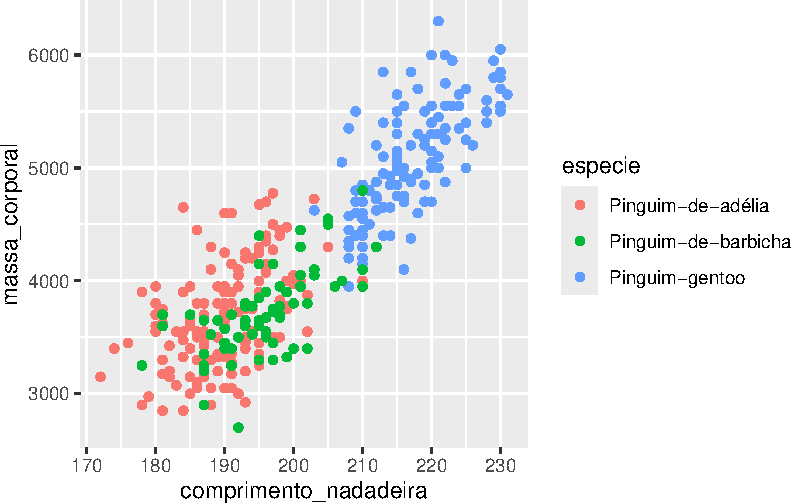
\includegraphics[keepaspectratio]{aula-2_files/figure-pdf/unnamed-chunk-3-1.pdf}}

\begin{Shaded}
\begin{Highlighting}[]
\FunctionTok{library}\NormalTok{(ggplot2)}

\FunctionTok{ggplot}\NormalTok{(dados}\SpecialCharTok{::}\NormalTok{pinguins) }\SpecialCharTok{+}
 \FunctionTok{aes}\NormalTok{(}\AttributeTok{x =}\NormalTok{ comprimento\_nadadeira, }\AttributeTok{y =}\NormalTok{ massa\_corporal, }\AttributeTok{colour =}\NormalTok{ especie) }\SpecialCharTok{+}
 \FunctionTok{geom\_point}\NormalTok{() }\SpecialCharTok{+}
 \FunctionTok{scale\_color\_brewer}\NormalTok{(}\AttributeTok{palette =} \StringTok{"Dark2"}\NormalTok{, }\AttributeTok{direction =} \DecValTok{1}\NormalTok{) }\SpecialCharTok{+}
 \FunctionTok{labs}\NormalTok{(}\AttributeTok{title =} \StringTok{"grafico"}\NormalTok{) }\SpecialCharTok{+}
 \FunctionTok{theme\_minimal}\NormalTok{()}
\end{Highlighting}
\end{Shaded}

\begin{verbatim}
Warning: Removed 2 rows containing missing values or values outside the scale range
(`geom_point()`).
\end{verbatim}

\pandocbounded{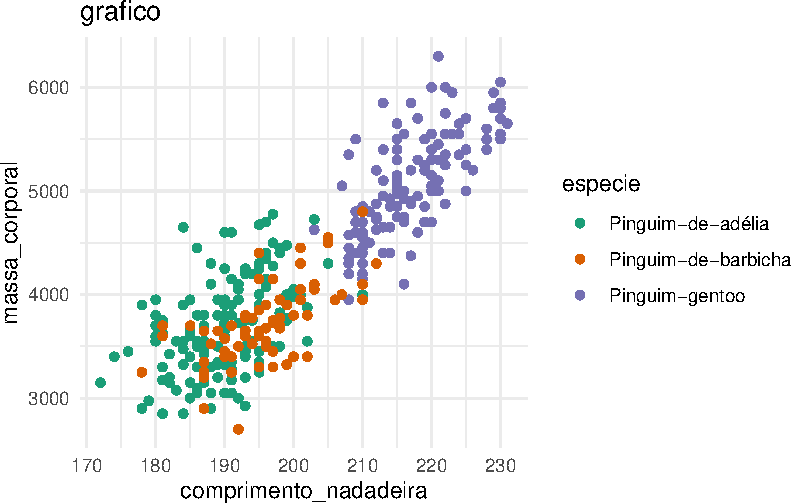
\includegraphics[keepaspectratio]{aula-2_files/figure-pdf/unnamed-chunk-4-1.pdf}}

\subsection{Código}\label{cuxf3digo}

\begin{Shaded}
\begin{Highlighting}[]
\FunctionTok{install.packages}\NormalTok{(}\StringTok{"esquisse"}\NormalTok{)}
\NormalTok{esquisse}\SpecialCharTok{::}\FunctionTok{esquisser}\NormalTok{()}
\end{Highlighting}
\end{Shaded}

\subsection{\texorpdfstring{Resultados de código no texto (\emph{inline
code})}{Resultados de código no texto (inline code)}}\label{resultados-de-cuxf3digo-no-texto-inline-code}

A base que utilizamos para análise tem 344 pinguins, de 3 espécies
diferentes: Pinguim-de-adélia, Pinguim-gentoo e Pinguim-de-barbicha. Os
pinguins foram amostrados nas seguintes ilhas: Torgersen, Biscoe e
Dream.

Os dados foram coletados entre 2007 e 2009.

A média do peso corporal é de 4.2 kg.

2025-01-16

\subsection{Nota de rodapé}\label{nota-de-rodapuxe9}

Quero escrever uma nota de rodapé\footnote{Essa é uma nota de rodapé.}.

\section{Imagens}\label{imagens}

\href{https://www.ime.usp.br/verao}{\begin{center}

\includegraphics[width=0.3\linewidth,height=\textheight,keepaspectratio]{aula-2_files/mediabag/logo_verao.png}
\end{center}
}

\begin{figure}[H]

{\centering \includesvg[width=0.3\linewidth,height=\textheight,keepaspectratio]{aula-2_files/mediabag/orcid.logo.svg}

}

\caption{Logo do ORCID}

\end{figure}%

\subsection{Para explorar nas próximas
aulas}\label{para-explorar-nas-pruxf3ximas-aulas}

\begin{itemize}
\item
  tabelas/quadro
\item
  imagens
\item
  tabelas sínteses de regressão. com o pacote stargazer
\item
  referências (elementos acadêmicos)
\item
  equações e expressões matemáticas com latex (elementos acadêmicos)
\item
  fluxograma - mermaid
\item
  mapas com leaflet
\end{itemize}




\end{document}
